\documentclass[10pt,aps,pra,onecolumn,superscriptaddress]{revtex4-1}

\usepackage{amsmath,amsthm}
\usepackage{amssymb}
\usepackage{amscd}
\usepackage{wasysym}
\usepackage[ansinew]{inputenc}
\usepackage[T1]{fontenc}
\usepackage{ae,aecompl}
\usepackage{hyperref}

   
    \usepackage[pdftex]{graphicx}
    \DeclareGraphicsExtensions{.pdf}

\usepackage{color}
\definecolor{red}{rgb}{1,0,0}
\definecolor{blue}{rgb}{0,0,1}
\definecolor{green}{rgb}{0,0.5,0}
\definecolor{magenta}{rgb}{1,0,1}

\newcommand{\marc}[1]{\textcolor{red}{#1}}
\newcommand{\dirk}[1]{\textcolor{blue}{#1}}
\newcommand{\debsankha}[1]{\textcolor{magenta}{#1}}
\newcommand{\ceil}[1]{\left\lceil#1\right\rceil}


% -- new commands -------------------------------------------

\newtheorem{thm}{Theorem}
\newtheorem{defn}[thm]{Definition}

\newcommand{\abs}[1]{\vert#1\vert}
\newcommand{\be}{\begin{equation}}
\newcommand{\ee}{\end{equation}}
\newcommand{\bea}{\begin{eqnarray}}
\newcommand{\eea}{\end{eqnarray}}
\newcommand{\nn}{\nonumber}
\newcommand{\ket}[1]{|#1\rangle}
\newcommand{\bra}[1]{\left\langle#1\right|}
\newcommand{\braket}[2]{\langle{#1}|{#2}\rangle}
\newcommand{\eye}{\mbox{$\mbox{1}\!\mbox{l}\;$}}
\newcommand{\E}{{\cal E}}
\newcommand{\N}{{\cal N}}
\newcommand{\EE}{\mathbf{E}}
\newcommand{\PP}{\mathbf{P}}
\newcommand{\HH}{\mathcal{H}}
\newcommand{\tr}{{\rm tr}}
\renewcommand{\vec}[1]{\boldsymbol{#1}}
\newcommand{\F}{{\cal F}}
\newcommand{\PR}{\mathcal{PR}}
\newcommand{\floor}[1]{\left\lfloor #1 \right \rfloor}
\newcommand{\maxp}{S(\vec{P})}
\newcommand{\maxf}{R(\vec{P})}

\newtheorem{lemma}{Lemma}
\newtheorem{theorem}{Theorem}
\newtheorem{corr}{Corollary}
\newtheorem{claim}{Claim}
\newtheorem{problem}{Problem}
\newtheorem{obs}{Observation}
\newtheorem{defi}{Definition}

% --- front matter ---------------------------------------------

\begin{document}
\bibliographystyle{apsrev}
\title{Geometric frustration and multistability in oscillator networks}

\author{Dirk Witthaut}
\affiliation{Network Dynamics, Max Planck Institute for Dynamics and Self-Organization (MPIDS), Am Fassberg 17, D--37077 G\"ottingen, Germany}

\author{Debsankha Manik}
\affiliation{Network Dynamics, Max Planck Institute for Dynamics and Self-Organization (MPIDS), Am Fassberg 17, D--37077 G\"ottingen, Germany}

\author{Who else}
\affiliation{Network Dynamics, Max Planck Institute for Dynamics and Self-Organization (MPIDS), Am Fassberg 17, D--37077 G\"ottingen, Germany}


\author{Marc Timme}
\affiliation{Network Dynamics, Max Planck Institute for Dynamics and Self-Organization (MPIDS), Am Fassberg 17, D--37077 G\"ottingen, Germany}
\affiliation{Faculty of Physics, Georg August University G\"ottingen,
  Germany}



\date{\today }


\begin{abstract}
We introduce the concept of geometric frustration for networks
of coupled oscillators. This concept readily explains some 
surprising features of the steady states of the network 
including Braess' paradox.
Using this approach  
we show that multistability is generally possible and derive
upper bounds for the number of stable steady states depending
on the network topology.
\end{abstract}


\maketitle

% --- Content --------------------------------------------------------------------

\section{Introduction}


\section{From Kuramoto oscillators to power grids}

Coupled oscillator models are ubiquitous in science and technology,
describing the collective dynamics of various systems form
the micro- to the macroscale. Research on coupled
oscillators dates back to Christian Huygens, who noticed that
two clocks synchronize when they are coupled \cite{Huyg93}.
One of the most important mathematical models was introduced
by Kuramoto \cite{Kura84} and succesfully applied
to describe the collective dynamics 
of coupled Josephson junctions \cite{Wies96}
neuronal networks \cite{Vare01}
chemical oscilaltors \cite{Kiss02}
and a variety of other synchronization phenomena
\cite{Stro00,Aceb05,Aren08},

The model describes the dynamics of the phases $\phi_j$
of $N$ coupled limit cycle oscillators 
\cite{Kura84},
$j = 1,\ldots,N$ is given by
\be
   \frac{d}{dt} \phi_j = \omega_j  + \sum_{\ell = 1}^N
      K _{j,\ell} \sin(\phi_\ell - \phi_j).
   \label{eqn:kuramoto}
\ee 


The coupling matrix $K$ is assumed to be symmetric.  It is useful to describe 
the system as a 
graph $G(V,E)$, whose vertex set $V$ is identical with the set of oscillator, 
and edge set $E$ is the set of all inter-oscillator couplings.  
%Then the graph 
%$G$ along with the natural frequencies $\omega_j$ contains all the information 
%needed to describe a Kuramoto system.   


A similar model of second-order oscillators describes
the collective phenomena of animal flocks \cite{Erme91,Ha10} or
human crowds \cite{Stro05} as well as the coarse-scale
dynamics of power grids
\cite{Fila08, 12powergrid,Mott13,Dorf13}.
In this 
model one considers $N$ coupled synchronuous machines, 
whose state is completely described by their mechanical 
phase $\phi_j$ and the phase velocity $\dot \phi_j$. The
acceleration (deceleration) of the machines is proportional
to the mechanical power $P_j$ generated (consumed) 
by the machine including friction losses. The detailed
equations of motion are derived from the conservation 
of energy with the result
\be
   \frac{d^2}{dt^2} \phi_j = P_j - \alpha \phi_j
             + \sum_{\ell = 1} K _{j,\ell} \sin(\phi_\ell - \phi_j). 
  \label{eqn:power}
\ee

The couplings $K_{j,l}$ has an additional interpretation: they are the 
admittance (inverse of the impedance) of the electrical transmission line 
joining node $j$ and node $l$.  

In this case the flow of electric power between the nodes
$\ell$ and $j$ is given by 
$F_{j,\ell}= K _{j,\ell} \sin(\phi_\ell - \phi_j) 
=  K _{j,\ell}  \Delta_{j,\ell}$.

Especially in the case of power grids, one is especially
interested in the existence of a globally phase-locked
solution, which describe the regular synchronous operation
of the machines. If this state is lost, some machines
will desynchronize with potentially catastrophic consequences.
In this paper we analyze the properties of the globally 
phase locked states of the oscillators which are defined
by $\phi_\ell - \phi_j = \mbox{constant}$ for all $(\ell,j)$
for both models. Without loss of generality, we can
assume that $\sum_j \omega_j = 0$ or
$\sum_j P_j = 0$, respectively,
such that the phase locked states correspond to the
stationary states of the system. Both for the Kuramoto
model and the power grid model, these states are given
by the solutions of the equations
\be
       \omega_j  + \sum_{\ell = 1}^N
      K _{j,\ell} \sin(\phi_\ell - \phi_j) =0 \qquad
     \forall j = 1,\ldots, N,
    %\label{eqn:sstate}
    \label{eqn:def-steady-state}
\ee
replacing $\omega_j$ by $P_j$ for the power grid.
In the following we anaylze the influence of the network
topology given by the coupling matrix $K_{j,\ell}$ on the
existence of a stationary state. Our results obviously hold
for both models, nevertheless our reasoning heavily relies
on the interpretation of $F_{j,\ell}= K _{j,\ell} \sin(\phi_\ell - \phi_j)$
as a flow which is inspired from the power grid model. 

One can generalize our results to include arbitrary coupling
functions $f$ instead of the sine (see, e.g., \cite{Wata93,Bick11}). 
In the following we mostly restrict ourselves to the common 
sine coupling for the sake of clarity.


%\textbf{XXX TO DO Revise and extend. Provide a short
%summary of the derivation of the oscillator model
%(Short means short - see for instance our PRL paper.)
%Mention classical model. Add a few words about
%the Kuramoto model in biological systems. 
%Add references. XXX}


\section{Role of network topology in stable operation}

\subsection{Completely coupled infinite dimensional systems}
\debsankha{I'm writing a summary of significant progress made so far on the 
topic of phase-locked operation of non-globally coupled Kuramoto oscillators.}

Numerous physical and biological systems are modelled by the Kuramoto model 
\eqref{eqn:kuramoto}. In 1975, Kuramoto made extensive research in \emph{completely coupled }
and \emph{infinite dimensional} systems with natural frequencies $\omega$ distributed according to a 
normalized pdf $g(\omega)$ satisfying $g(\omega)=g(-\omega)$.  He showed that in those systems, a phase transition occurs 
when the uniform global coupling $K$ is increased gradually. To this end, he 
defined the \emph{order parameter} $r$
\begin{equation}
\label{eq:kuramoto_r}
re^{i\Psi}=\frac{1}{N}\sum_j e^{i\theta_j}. 
\end{equation}

At low $K$, the 
oscillators are uniformly distributed on 
the unit circle.  However, after a critical coupling, 
$K>K_c=\frac{2}{\pi g(0)}$, a \emph{partial phase locking happens:} all 
oscillators with $-Kr<\omega<Kr$ phase lock such that
\begin{equation}
Kr\sin{(\theta-\Psi)}=\omega.  
\end{equation}

As $K$ is increased further, $r$ keeps increasing: and therefore, more 
oscillators enter the phase locked state from the incoherent state.  If the 
frequency distribution $g(\omega)$ has a bounded support, there exists a 
$K_{lock}>K_c$ at which all the oscillators phase lock.  At the 
$K\gtrapprox K_c$ limit, there exists a scaling law
\begin{equation}
\label{eq:kuramoto-scaling}
r\sim\sqrt{\frac{-16(K-K_c)}{\pi K_c^4g''(0)}}. 
\end{equation}
As we can see from \eqref{eq:kuramoto-scaling}, if $g(\omega)$ is \emph{curved 
upward}, this law gives nonsensical results.   Apparently there will be a \emph{supercritical} phase transition 
\cite[p.~6]{acebron2005kuramoto}: there will be  co-existence of $r=0$ phase 
and $r>0$ phase \emph{before} $K=K_c$.  

\section{The nature and bifurcations of steady states}
\textbf{XXX TO DO: Please provide a short summary of
our EPJ ST paper.}


Both the Kuramoto system and the oscillator model of 
power grid share the same set of fixed points as described by \eqref{eqn:def-steady-state}. It has been shown 
\cite{epjst14} that the similarity between these two systems runs 
deeper, namely, the stability properties of those fixed points are also identical 
for the two systems.  As a consequence, they both have the same bifurcation structure.   

\subsection{Local and global stability}
The stability analysis for both the systems at a certain fixed point 
$\vec{\theta^*}=(\theta_1^*,\ldots,\theta_N^*)$ can be performed easily by 
defining the potential function

\begin{align}
\label{eq-potential}
V(\theta_j)=- \sum_j P_j \theta_j - \frac{1}{2} \sum_{i,j} K_{ij} \cos(\theta_i - \theta_j).
\end{align}

The fixed points can be shown to be local extrema of this potential.  For any 
fixed point $\vec{\theta}^*=(\theta_1,\theta_2,\cdots,\theta_n)$, it
is asymptotically stable if the Hesse matrix $M$ of the potential 
function 
\begin{align}
\label{eq-M}
   M(\vec{\theta^*})&=\begin{pmatrix}
      \sum_l K_{1l} \cos{(\theta_1^*-\theta_l^*)} & 
              - K_{12}\cos{(\theta_1^*-\theta_2^*)} & \cdots \\
     - K_{21}\cos{(\theta_2^*-\theta_1^*)} & 
               \sum_l K_{2l} \cos{(\theta_2^*-\theta_l^*)} & \cdots \\
       \vdots & \vdots  & \ddots 
  \end{pmatrix}
\end{align}
has eigenvalues positive.  It is worth noting, that $M$ has one eigenvector 
$\vec{v}_1=(1,1,\cdots,1)$ with eigenvalue $0$, but this is merely an artifact 
of the fact that any fixed point $\vec{\theta^*}$ is arbitrary upto an 
additive constant.  

\begin{claim}
Let the eigenvalues of $M$ be $0=\mu_1\leq\mu_2\leq\cdots\leq \mu_N$.  If for a given network topology and a given fixed point, 
 \[
\mu_k\ge 0,\quad\forall k=2,3,\cdots,N
 \]
then that fixed point is \emph{asymptotically stable} for both 
Kuramoto system and the power grid model system.  
\end{claim}

\subsection{Bifurcation and loss of stability}
Using some results from bifurcation theory, it has been shown in
\cite{epjst14} that a stable fixed point can only be lost by an inverse 
saddle-node bifurcation when one of the eigenvalues $\mu_k$ becomes zero.  

When the phase differences across all edges in the network are sufficiently 
small such that
\begin{align}
\label{def:normal-op}
\cos{\left(\theta_i^*-\theta_j^*\right)\ge 0}
\end{align}
for all edges $(i,j)$ in the network, it is said to be in the \emph{normal 
operation}. More insights can be gained about the loss of a steady state when 
the network is in the normal operation.  

For a powergrid under normal operation, we can define a \emph{meta graph} 
$\tilde{G}(V,\tilde{E})$ whose vertices are the oscillators, as in $G$, but the
edges have weights
\begin{align}
\label{gtilde-weights}
K_{jl}\cos\left(\theta_l-\theta_j\right).
\end{align}

Then the matrix $M$ as defined in \eqref{eq-M} is seen to be 
the Laplacian matrix of the meta graph $\tilde{G}$. It follows from graph 
theory that an eigenvalue of $M$ can become $0$ only when $\tilde{G}$ 
disconnects into two (or more) components.  It can be easily seen from 
\eqref{gtilde-weights} that such a split-up happens only when all the 
transmission lines
connecting two certain parts (denoted by $G_1, G_2$) of the network are completely saturated
\begin{align}
\label{}
\abs{\theta_j-\theta_l}&=\frac{\pi}{2},\quad\forall (j,l)\in E, j\in G_1,l\in 
G_2. 
\end{align}

\dirk{XXX General note: Include the new references to the reference list. XXX}

\section{Geometric frustration}
\label{sec:frustration}


It is instructive to divide the defining equation 
(\ref{eqn:def-steady-state}) of an 
equilibrium state into two parts.
First, every stationary state has to satisfy a dynamic condition 
which is nothing but the conservation of the flow at every node
of the network
\begin{subequations}
\label{eqn:dc1}
\begin{align}
   & P_j + \sum_{\ell=1}^N K _{j,\ell} S_{j,\ell} = 0 \qquad 
              \forall j=1,\ldots,N. \\
  &  |S_{j,\ell}|   \le 1 \quad \qquad \qquad \qquad  
              \forall \; \mbox{edges} \, (j,\ell).
\end{align} 
\end{subequations}
Here, $\sum_\ell K_{j,\ell}S_{j,\ell}$ is the sum of all 
flows from the neighboring nodes to the node $j$, while 
$P_j$ is a source or sink term, respectively.
The second part of this condition reflects the fact that the
transmission capacity of each link is bounded, such that the
magnitude of the flow $|F_{j,\ell}|$ cannot exceed the capacity
$K_{j,\ell}$.  
The dynamic condition (\ref{eqn:dc1}) hold for
all flow networks including also DC networks (i.e. Kirchhoff's
rules) and biological network models \cite{Kati10}. 

To obtain a better understanding of the possible solutions,
we slightly rephrase the dynamic condition  (\ref{eqn:dc1}).
To this end we label all the edges in the network with $e = 1,\ldots,L$.
As the flows are directed, we have to keep track of the ordering
of the vertices connected by the edge $e$. That is, each $e$ 
corresponds to a directed link $(j,\ell)$ in the following. The ordering
is arbitrary but must be kept fixed.
Then we write $S_e = S_{j,\ell}$ and $F_e = F_{j,\ell}$
for the flow over a link $e  \,  \widehat= \, (j,\ell)$. 
Furthermore, we define the edge incidence matrix
$\widetilde K \in \mathbb{R}^{N\times L}$ via
\be
   \widetilde K _{j,e} = \left\{
   \begin{array}{r l }
      K_{j,e} & \; \mbox{if node $j$ is the head of edge $e  \,  \widehat= \, (j,\ell)$},  \\
      - K_{j,e} & \; \mbox{if node $j$ is the tail of edge $e  \,  \widehat= \, (j,\ell)$},  \\
      0     & \; \mbox{otherwise}.
  \end{array} \right.
\ee
The dynamic condition (\ref{eqn:dc1}) then reads
\begin{subequations}
\label{eqn:dc2}
\begin{align}
   & P_j + \sum_{e=1}^L \widetilde K _{j,e} S_e = 0 \qquad 
              \forall j=1,\ldots,N. 
     \label{eqn:dc2a}  \\
  &  |S_{e}|   \le 1 \quad \qquad \qquad \qquad  
              \forall e = 1,\ldots,L.
  \label{eqn:dc2b}
\end{align} 
\end{subequations}
Here $\vec S = (S_1,\ldots,S_L)^t$ is a vector in $\mathbb{R}^L$
The rank of $\widetilde K$ is $(N-1)$ such that the solutions 
of the linear set of equations (\ref{eqn:dc2a}) span an afine 
subspace of $\mathbb{R}^L$ whose dimension  is $(L-N+1)$. 
Physically speaking, the dynamical condition is just the
conservation of flow at each node. The homogeneous 
solutions of the system (\ref{eqn:dc2a}) are just the cycle
flows which do not affect flow conservation. As the number
of fundamental cycles in a network is  $(L-N+1)$, the dimension
of the solution space is also given by $(L-N+1)$.
The condition (\ref{eqn:dc2b}) defines a bounded convex 
polytope in $\mathbb{R}^L$. Physically speaking, this condition
ensures that no link is overloaded. 
In many important applications $L$ is much larger than 
the number of nodes $N$, such that the dynamical
conditions typically yield a large submanifold of solutions
as candidates for equilibrium states. However, the set of
solutions can also be empty if the capacities $K_{j,\ell}$
are too small such that the polytope does not intersect
the afine subspace.
  

Second, there is a geometric condition.  We state the conditions as follows.
A stationary state exists if the flows 
$F_{j,\ell} = K_{j,\ell} S_{j,\ell}$
satisfy the dynamical conditions (\ref{eqn:dc1}) 
\emph{and if}  
\bea
    \exists \, \theta_j \quad \mbox{such that}  \;
    S_{j,\ell} = \sin(\theta_\ell - \theta_j).
  \label{eqn:gc1}
\eea
We note that there are always two solutions for the phase 
difference $\Delta_{j,\ell} = \theta_j - \theta_\ell$ 
for a given value of $S_{j,\ell}$:
\bea
     && \Delta_{j,\ell}^+ = \arcsin(S_{j,\ell}) 
      \qquad \mbox{or} \nn \\
    && \Delta_{j,\ell}^- = \pi -  \arcsin(S_{j,\ell}),
     \label{eqn:deltaS} 
\eea
which both have to be considered in principle. A solution
where the $+$-sign is chosen for all edges is guaranteed 
to be stable if it exists, see corrolary \ref{corr:stab-phasediff}.
The converse statement is not generally true
[Manik 2014].

We now rephrase this condition in a more instructive way.
To this end we assume that we have already obtained a solution
of the dynamic conditions (\ref{eqn:dc1}). Then we can try to
succsesively assign a phase $\theta_j$ to every node $j$ in the
network. Starting at a node $j_0$ with an arbitrary phase
$\theta_{j_0}$, we assign the phases of all neighboring nodes
$j_1$ such that $\sin(\theta_{j_1}   -   \theta_{j_0}) = S_{j_0,j_1}$.
We then proceed in this way through the complete network
to assign the phase of an arbitrary node $j_n$,
\be
   \theta_{j_n} = \theta_{j_0} + \sum_{s=0}^{n-1}
      \Delta_{j_s,j_{s+1}},
   \label{eqn:phase-path}
\ee
where $(j_0,j_1,\ldots,j_n)$ is an arbitrary \emph{path} form
$j_0$ to $j_n$. 
In the general case, however, a given node $j_n$ can be reached
from $j_0$ via a multitude of different paths. To define a unique
set of phases that satisfies the geometric condition (\ref{eqn:gc1}),
we must assure that Eq.~(\ref{eqn:phase-path}) yields a unique 
phase regardless which path is taken from $j_0$ to $j_n$.
This is equivalent to the condition, that the phase 
differences over every \emph{cycle} in the network 
must add up to an integer (the \emph{winding number}) times $2\pi$.  
\bea
       \label{eqn:gc2}
    && \sum_{\rm cycle} \Delta_{j,\ell} = 2 m \pi,\quad, m\in\mathbb{Z}
\eea
where $\Delta_{j,\ell}$ is one of the solutions defined in 
Eq.~(\ref{eqn:deltaS}). 
Furthermore, one only has to consider the fundamental
cycles of the network which form a basis for the cycle space.
If Eq.~(\ref{eqn:gc2}) is satisfied for all fundamental cycles, it is 
satisfied for all simple cycles of the network.
Thus, we can refomulate the conditions for the
existence of a stationary state (\ref{eqn:def-steady-state}) 
as follows.

\begin{thm}
A stationary state exists if the flows 
   $F_{j,\ell} = K_{j,\ell} S_{j,\ell}$
satisfy the dynamics conditions (\ref{eqn:dc1})  and if
the geometric condition (\ref{eqn:gc2}) is satisfied for
all fundamental cycles in the network.
\end{thm}


%\section{Geometric frustration}

The previous reasoning shows that we can face the following
situation: Given an oscillator network characterized by the
frequancies $P_j$ and the capacity matrix $K_{j,\ell}$,
we can find a solution of the dynamical conditions, such that
the flow is conserved at all nodes of the network. Nevertheless,
no equilibrium state exists as these solutions are incompaticle 
to the geometric conditions. In this case we say that phase
locking is inhibited due to geometric frustration. We 
summarize this in a formal definition before giving some
examples for the importance of this phenomenon. 


\begin{defn}
An oscillator network is said to be {geometrically 
frustrated} if a solution of the dynamic conditions 
(\ref{eqn:dc1}) exits, but all solutions are incompatible
to the geometric conditions (\ref{eqn:gc2}) such 
that no equilibirum state exists.
\end{defn}


This definition seems unfamiliar thinking of the common examples 
of geometric frustration in condensed matter theory. However, it is 
completely compatible to more general definitions based on probability
theory (see, e.g., \cite{Wolf03}). In such a generalized framework
geometric frustration in defined as follows.
Given $N$ (stochastic) variables $x_1,\ldots,x_N$ and $L$ pair
distribution or correlation functions $P(x_j,x_\ell)$. The main question 
is: Is there a joint probability distribution $P(x_1,\ldots,x_N)$ which
yields all the pair distribution functions as marginals? If such
a distribution does not exist, the system is called gemotrically
frustrated. Our definition is a direct concretisation of this
general definition. For each edge $(j,\ell)$ of the network, the 
dynamical condition (\ref{eqn:dc2a})  yields a correlation function for the phases
$\theta_j, \theta_\ell$ of the adjacent nodes. The main question is 
whether there correlations are compatible such that we can 
find a unique set of phases.

\section{Examples and applications}

In this section we discuss the importance of geometric aspects 
for the stationary states of an oscillator network with different
topologies. In particular, we analyze the number of equilibrium
states and show that geometric frustration can inhibit phase 
locking, which may lead to a very counter-intuitive effects.


\subsection{Trees do not suffer from frustration.}

By definition, a tree does not contain any cycle such that
the geometric condition (\ref{eqn:dc1}) does not apply. 
Therefore, the calculation of an equilibrium state  of the 
power grid oscillator model and the Kuramoto model 
as defined by Eq.~(\ref{eqn:def-steady-state})
on a tree reduces to the solution of the dynamic condition 
(\ref{eqn:gc2}), which is a linear set of equations. 
Moreover, we can find a strong result on the 
the number of stable and unstable equilibrium 
states -- see corrolary \ref{eqn:corr-tree}.



\subsection{Multiple solutions in cycle}

We now consider the simplest case of a cyclic network with only 
three nodes and three links with equal strength $K$. The 
dynamical condition for the existence of an equilibrium state then
reads
\be
   K \begin{pmatrix} 0 & 1 & -1 \\ -1 & 0 & 1 \\ 1 & -1 & 0   
   \end{pmatrix}
   \begin{pmatrix} S_{12} \\ S_{23} \\ S_{31} \end{pmatrix}
  = \begin{pmatrix} P_3 \\ P_1 \\ P_2 \end{pmatrix}
    \label{eqn:3cycle-dc} 
\ee
 and $|S_{j,\ell}| \le 1$. In particular for $P_j = 0$ the
set of possible solutions is just the a cycle flow 
$(S_{12}, S_{23}, S_{31}) = S \times (1,1,1)$.

Taking into account that there are two possible solutions for the
phase difference, see Eq.~(\ref{eqn:deltaS}), the geometric condition
can be written as
\bea
      \arcsin(S_{12}) + \arcsin(S_{23}) +  \arcsin(S_{31}) &=& 0    \nn \\ 
      \arcsin(S_{12}) + \arcsin(S_{23})  -  \arcsin(S_{31}) &=& \pi \nn \\ 
      \arcsin(S_{12}) - \arcsin(S_{23})  + \arcsin(S_{31}) &=& \pi \nn \\ 
   - \arcsin(S_{12}) + \arcsin(S_{23})  +  \arcsin(S_{31}) &=& \pi  
   \label{eqn:3cycle-gc} 
\eea 
Figure \ref{fig:cycle3} shows the affine set defined by 
Eq.~(\ref{eqn:3cycle-dc})  and one branch of the solution
space defined by  (\ref{eqn:3cycle-gc}). One observes that 
there are three intersections corresponding to 
three stationary states. This shows that stationary
states are generally not unique, also in the presence
of cycles.
The three remaining branches of the solution space
of Eq.~(\ref{eqn:3cycle-gc}) do not yield additional
solutions.
In the present case only one of the solutions are stable,
but this is generally not true in larger cycles as we will
show in the following.


\begin{figure}[tb]
\centering
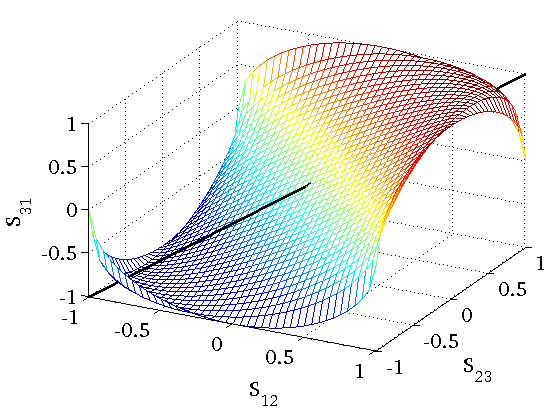
\includegraphics[width=8cm, angle=0]{pics/cycle3b.png}
\caption{\label{fig:cycle3}
Geometric solution of the simplest cyclic network with
3 nodes with $P_j=0$ and three links with equal
strength $K$.
The black line is the solution space of the dynamical 
condition (\ref{eqn:3cycle-dc}) and the surface is the
relevant branch of the solution space of the geometrical
condition (\ref{eqn:3cycle-gc}). One finds three intersections 
corresponding to three stationary states.
}
\end{figure}

\subsection{Frustration induces discreteness.} 
\label{eqn:sec-cycle}

We now extend the above example to a single cycle with an
arbitary number of $N$ nodes with  the same power
$P_j \equiv 0$. All links have an equal strength $K$ as above.
The dynamic conditions for a stationary states are then given by
\bea
  && F_{j+1,j} = F_{j,j-1}  \equiv F \qquad \forall j = 1,\ldots,N  \\ 
  && |F| \le K.
\eea
For notational convenience we identify the node $1$ with $N+1$ and
$0$ with $N$.  The geometric condition yields
\bea
   && N \mbox{arcsin}(F/K) = 0 \quad (\mbox{mod} 2 \pi) \nn  \\
   \Rightarrow \, &&  F = K \sin(2\pi n/N), \qquad  n \in \mathbb{Z}\ \\  
   \Rightarrow \, && \, \theta_{j+1} - \theta_j = \frac{n}{N} 2 \pi .
\eea
This shows that the dynamic condition has a continuum of 
solutions while the geometric condition induces a 
quantization of the phase differences 
$\theta_{j+1} - \theta_j$. 

\dirk{XXX We don't even get all states here because I had implicitly assumed
that $\theta_{j+1} - \theta_j$ is the same for all $j$. Fix the example! XXX}

In total we find $N$ different stationary states of this kind
with $n = 0,\ldots,N-1$,
taking into account that the phases are only defined modulo
$2\pi$. The eigenvalues of the Hesse matrix $A$ are given
by
\be
     \mu_k = -4 K \cos(2\pi n/N) \sin^2(\pi k/N),
        \; k = 1,\ldots,N. \nn
\ee
Therefore we find that all equilibria with 
$n \in [0,N/4]$ or $n\in[3N/4,N]$ are dynamically 
stable.
 

This example is very simple but shows three important results
of ours most clearly which hold in general.
First, there can be \emph{multiple} stable equilibrium states in cyclic
networks as previously noticed by [Ochab+Gora, Taylor, HMO]. This fact is not
fully recognized in the power engineering, probably because most 
authors in this community concentrate of connected networks
(see, e.g.~\cite{Mach08}).
Second, the oscillator model (\ref{eqn:power}) allows for 
stable equilibrium states with a persitent current around a cycle.
Interestingly, theses states are phase locked but \emph{not phase
ordered} in the sense that the phase order parameter
\cite{Stro00}
\be
   r e^{i \psi} := \frac{1}{N} \sum_j e^{i \theta_j} 
   \label{eqn:deforder}
\ee
vanishes exactly.
Third, the geometric condition induces the 
\emph{discreteness} of the phase differences
although the dynamic condition allows for continuous
values of cycle flows.


\subsection{Braess' paradox}
\label{sec:braess}

Here we introduce a special example which illustrates the
paradoxial efffects of geometric frustration most clearly.
We consider the oscillator network depicted in Fig.~\ref{fig:braess} (a)
consisting of $N=6$ nodes placed on a cyclic network.
In particular, we analyze what happens if the capacity
of the upper edge is increased from $K$ to 
$K' = K + \kappa$. 


\begin{figure}[tb]
\centering
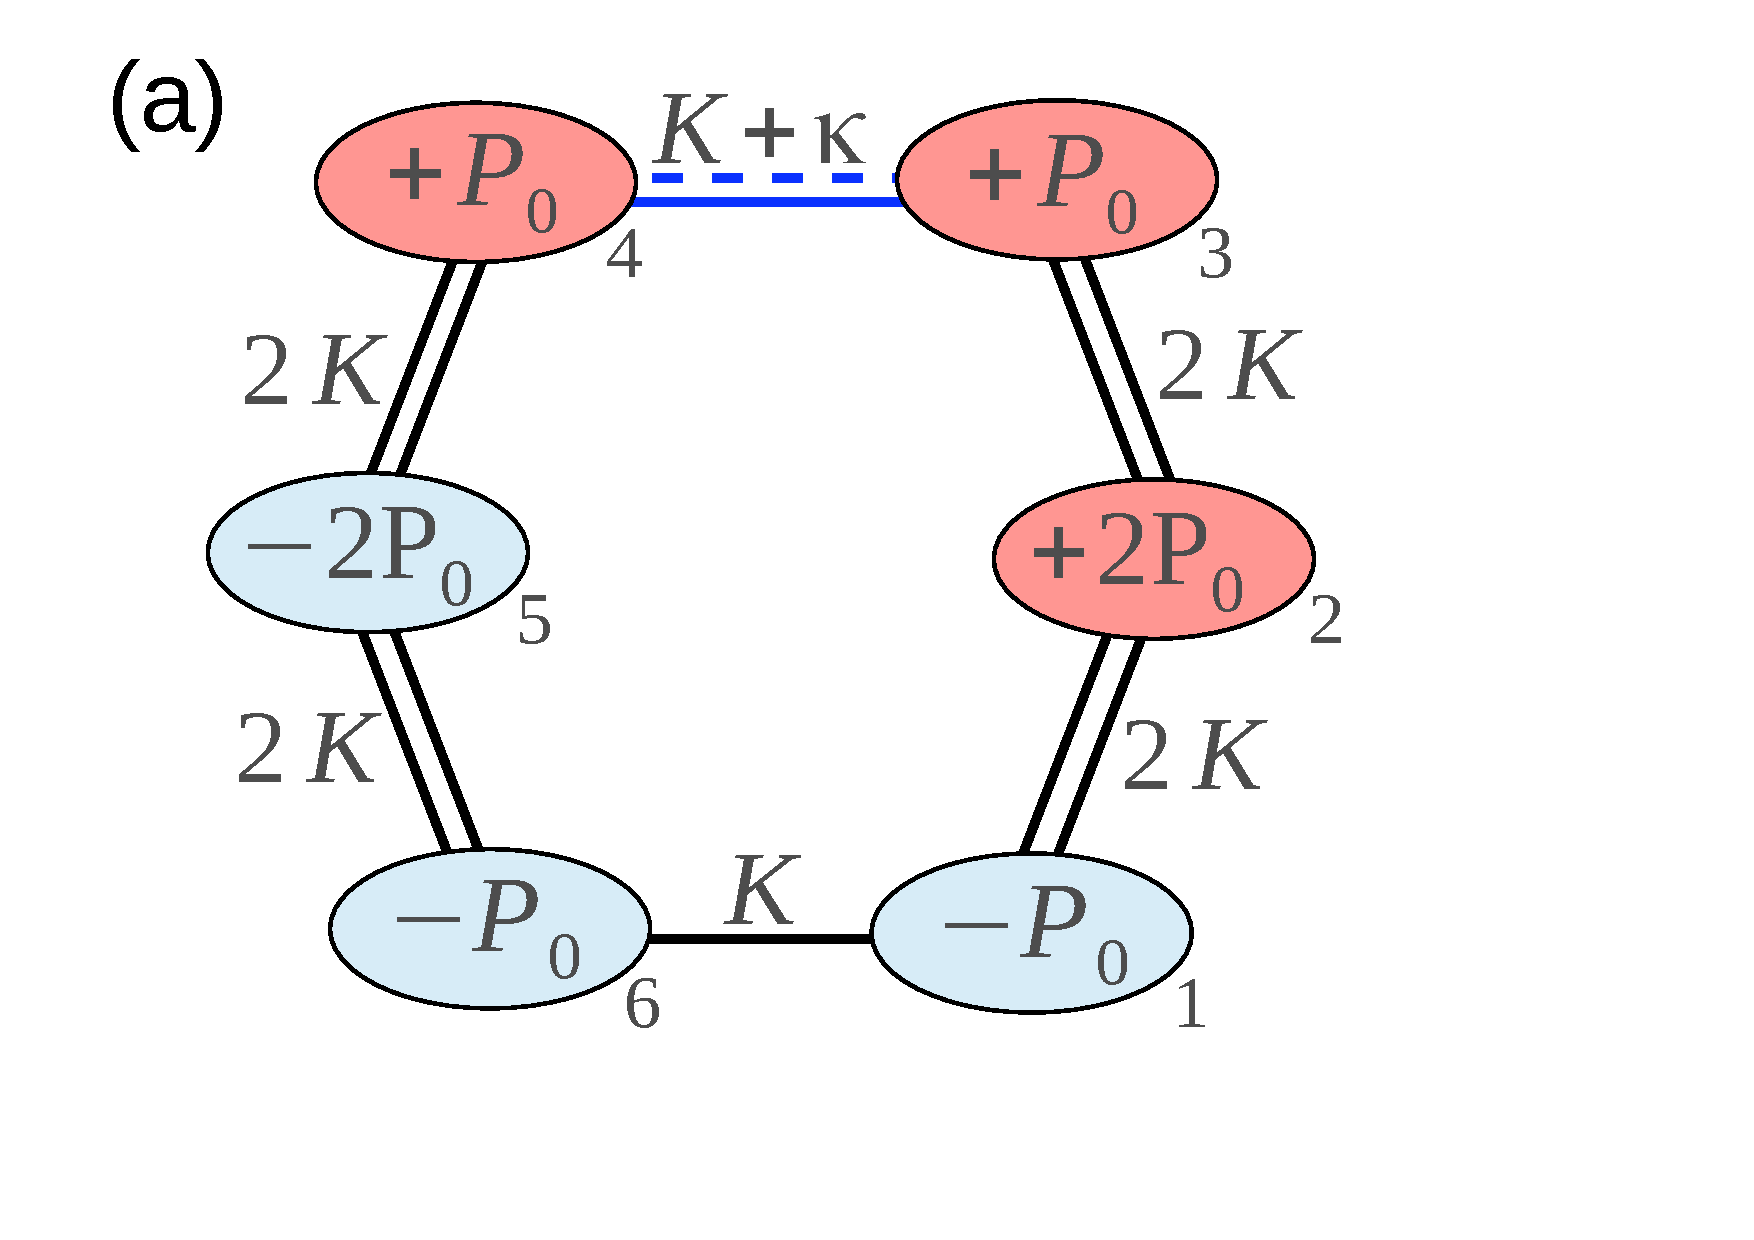
\includegraphics[width =3.6cm, angle=0]{pics/cycleex1_a}
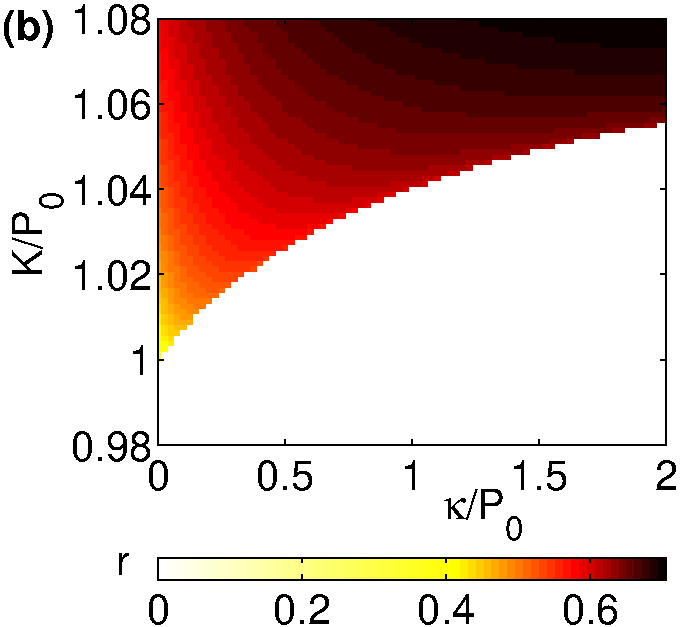
\includegraphics[width=4.3cm, angle=0]{pics/braess_order3}
\caption{\label{fig:braess}
Geometric frustration induces Braess' paradox.
(a) Topology of the network under consideration.
(b) Stability phase diagram: Order parameter $r$ 
as a function of $K$ and $\kappa$. No equilibrium 
state exists in the white region. 
The equilibrium can be lost when the
local transmission capacity $\kappa$ 
\emph{increases}.
}
\end{figure}

The dynamic condition for this network reads
\be
   0 = P_j + ( K_{j+1,j} S_{j+1,j}  - K_{j,j-1} S_{j,j-1} ),
   \label{eqn:dc-braess}
\ee
and $|\Delta_{j,j+1}| \le 1$, identifying node $j=7$ with $j=1$.
 For notational convenience,
we define the vector 
\be
   \vec S = (S_{6,1} ,S_{1,2}, \ldots, S_{5,6} ).
\ee
The solutions of the linear system of equations (\ref{eqn:dc-braess}) 
span a one-dimensional affine space parametrized by a real 
number $\epsilon$,
\be
   \vec S = \frac{P_0}{K} 
      \left( \vec S_a - \epsilon \, \vec S_b \right).
   \label{eqn:SaSb2}
\ee
The vector $\vec S_a = (1,1,0,-K/K',-1, 0)$ is the 
inhomogeneous solution of the linear system (\ref{eqn:dc-braess}), 
and the vector $\vec S_b = (2,1,1,2K/K',1,1)$is a homogeneous 
solution corresponding to a cycle flow.
Evaluating the condition $|S_{j,j+1}| \le 1$ yields
a necessary condition for the existstence of a stationary state
\be
     K \ge P_0.
\ee

For $\kappa = 0$ this condition is also sufficient for
the existence of a stationary state. If the capacity of the
upper link increases, $\kappa > 0$, geometric frustration
inhibits phase locking. A solution of the dynamical conditions
always  exists for   $K \ge P_0$, but this can become 
incompatible with the geometrix condtion as illustrated 
in the stability diagram  in Figure \ref{fig:braess} (b). No equilibrium
state exists in the white region of parameter space. 
In the remaining region, we have plotted the Kuramoto phase 
order parameter (\ref{eqn:deforder})
in a color color.
One clearly observes that the unstable region \emph{increases} 
with $\kappa$. This leads to the paradoxial effect that
an increase of local transmission capacity reduces
the ability of the network to support a phase locked 
equilibrium state. This behavior can also be seen as an example of 
Braess' paradox which has been first predicted for traffic 
network \cite{Brae68,12braess}.
 

\section{Multistability and the number of equilibria}

The previous examples show that there can be quite a large
number of stable equilibrium states in a cyclic network. 
In the following we derive bounds on the number of stable 
equilibria for depoending on the network structure.

\subsection{Tree network}

In the previous section we have argued that multistability
arises due to the possibility of cycle flows. In a tree there
are no cycles such that we obtain the following very strong result.

\begin{corr}
\label{eqn:corr-tree}
In a tree network, there is either no equilibrium state
or there are $2^{N-1}$ equilibrium states of which
one is stable and $2^{N-1}-1$ are unstable.
\end{corr}

\begin{proof}
By definition, a tree has $L=N-1$ edges such that the
space of solutions of the linear system (\ref{eqn:dc2a}) 
has dimension $L-N+1 = 0$. That is, there is either zero
of exactly one unique solution for the flows $F_{j,\ell}$.
In the first case no equilibrium exists. In the latter case
there are $2$ possible values for the phase difference 
for each of edge given by equation (\ref{eqn:deltaS}).
Hence there are $2^L = 2^{N-1}$ equilibrium states.
Choosing the $+$-sign in equation (\ref{eqn:deltaS}) 
yields one stable equilibrium state as shown in corrolary 
\ref{corr:stab-phasediff}.

It remains to show that all other equilibrium states are unstable.
So consider an equilibrium state with one edge with a phase difference 
that exceeds $\pi/2$. The network is a tree such that it is decomposed
into two parts which are only connected by this edge. We label the
nodes by $1,\ldots,\ell$ in one part and by $\ell+1,\ldots,N$.
in the other part. Then the Hesse matrix $A$ has the form
\be
    A  = \left( \begin{array}{c|c}
    A_1 & 0     \\   \hline
    0 & A_2 \\ 
   \end{array} \right) +
    \begin{pmatrix}
       \ddots & & & & \\
       & 0 &0 & 0 & 0 &  \\
        & 0 & K^{\rm red}_{\ell,\ell +1} & -K^{\rm red}_{\ell,\ell +1} & 0 & \\
        & 0 & -K^{\rm red}_{\ell,\ell +1} & K^{\rm red}_{\ell,\ell +1} & 0 & \\
       & 0 & 0 & 0 & 0 & \\
      &  &  & & & \ddots \\
  \end{pmatrix}, \nn
\ee
where $K^{\rm red}_{\ell,\ell +1} < 0$
and $A_1$ and $A_2$ are defined as in equation
(\ref{eqn:def-hesse}) for the two parts of the network.
Now define the vector
\be
   \vec v = ( \underbrace{1,\ldots,1}_{\ell \, {\rm times}},
                     \underbrace{0,\ldots,0}_{(N-\ell) \, {\rm times}} )^T.
\ee
Due to the structure of the matrix $A_1$ we have 
$A_1 (1,\ldots,1)^T = \vec 0$ such that
\be
   \vec v^T A \vec v =  K^{\rm red}_{\ell,\ell +1} < 0.
\ee
Thus, the Hesse matrix $A$ is not positive semi-definite, 
i.e.~it has at least one negative eigenvalue and the 
equilibrium state is unstable (cf.~observation \ref{eqn:obs-lam-mu}).
\end{proof}

\subsection{Simple cycles}
\label{sec:cycles}

For networks containing a single cycle, it is possible to derive rather
tight upper and lower bounds for the number of steady states which satisfy
\begin{align}
\label{def:normalop}
|\theta_i^*  - \theta_j^*| \le \pi/2
\end{align}
for all edges $(i,j)$. These states are
guaranteed to be stable by corollary XXX. They correspond to the normal
operation of a power grid. Other stable steady states can exist in particular
at the border of the stable parameter region [Malik 2014].  


\begin{defn}
For a ring network $R_N$ with $n\in \mathbb{N}$ nodes indexed by $1,2,\cdots,N$, a \textbf{fragment} $R_{i,j}$ is 
defined as the path starting at node $i$ and ending at node $j$:
	\[
         R(i,j)=(i,i+1,\cdots, j)
	\]
It is to be noted that we identify node $1$ with $N+1$ and so on.   

For any ring fragment $R_{i,j}$, the \textbf{partial net power} $\bar{P}_{ij}$ is defined as
\[
\bar{P}_{ij}=\sum_{k\in R(i,j)} P_k.  
\]
\end{defn}


\begin{lemma}
\label{lem:flow-power}
For any ring fragment $S_{i,j}$, the partial net power is equal to the net outwards flow:
\begin{align}
\label{eq:glow-power}
\bar{P}_{ij}=F_{j,j+1}-F_{i-1,1}
\end{align}
\end{lemma}

\begin{proof}
Conservation of energy.  
\end{proof}

\begin{figure}[!htp]
\caption{$\bar{P}_{\max}$ in different rings}
\label{fig:pmax}
\begin{center}
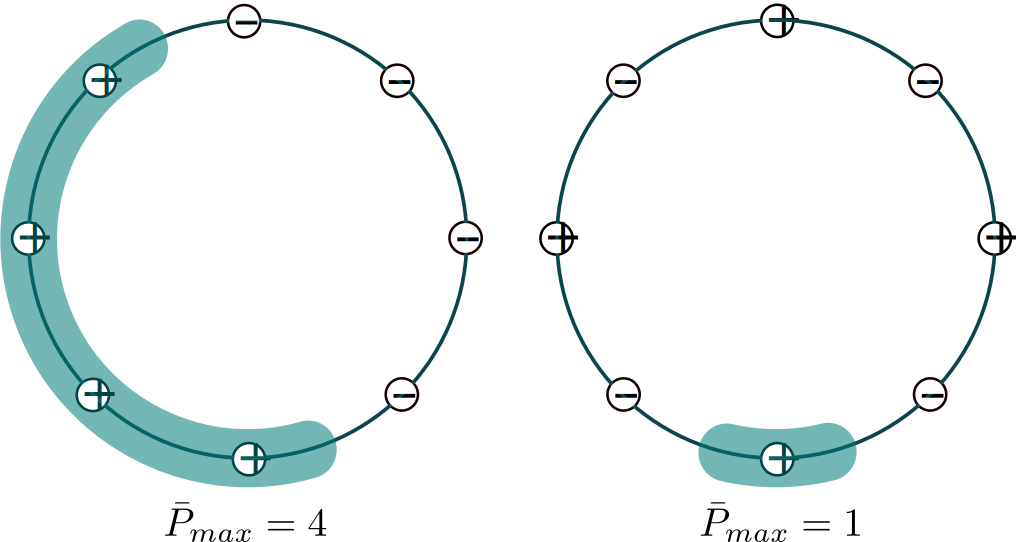
\includegraphics[width=0.6\columnwidth]{pics/pmax_compare}
\end{center}
\end{figure}


\begin{defn}
For any ring network $R$, the \textbf{maximal partial net power} is defined as
\begin{align}
\label{def:mpnp}
\bar{P}_{\max}=\max_{i,j} \bar{P}_{i,j}
\end{align}
This concept is illustrated in Fig.\ref{fig:pmax}
\end{defn}


\begin{lemma}
\label{lem:cf-fp-corr}
Let $\vec{\phi_0}$ is a fixed point of a ring network $R$.  Then any other 
fixed point $\vec{\phi_k}$ of the same network must differ from $\vec{\phi_0}$ 
by a \emph{cycle flow} $f^{cycle}(k)$.  

In other words, if $\mathbf{S}_R$ be the set 
of all fixed points of a ring network $R$, there exists a one-to-one 
function $f^{cycle}:\mathbf{S}_R\mapsto \mathbf{R}$. 
\end{lemma}

\begin{proof}
If $|\mathbf{S}_R|<2$  the Lemma is vacuously true.  
Suppose $\vec{\phi_0},\vec{\phi_1} \in \mathbf{S}_R$.   

Let $(F^0_1, F^0_2,\cdots,F^0_N)$ and $(F^1_1, F^1_2,\cdots,F^1_N)$ be the flows 
associated with $\vec{\phi_0}$ and $\vec{\phi_1}$.  

Using Lemma \ref{lem:flow-power}, we see that
\begin{align}
\label{}
F_{j,j+1}-F_{i-1,j}&=P_j\quad\forall j \\
F'_{j,j+1}-F'_{i-1,j}&=P_j
\end{align}

Therefore
\begin{align}
\label{}
F^0_{j,j+1}-F^1_{j,j+1}&=F^0_{j-1,j}-F^1_{j-1,j}=c,\quad\forall j\\
\Rightarrow F^0_{j,j+1}-F^1_{j,j+1}&=c,\quad\forall j.   
\end{align}
So all the flows in the second steady state differs from the first one by a 
constant amount $c$.   

So the function $f_c(\phi_m)=F^m_{j,j+1}-F^0_{j,j+1}$ is by construction a 
one-to one function mapping each fixed point to a cycle flow.  
\end{proof}



\begin{defn}
For any ring network $R$ and a fixed point $\vec{\phi}$, the \emph{winding 
number of the fixed point} is defined as 
\begin{align}
\label{def:wnum}
\omega(\vec{\phi})&=\frac{1}{2\pi}\sum_{\text{all edges }e} \arcsin{\frac{F_e}{K_e}}\\
&=\frac{1}{2\pi}\sum_{\text{all edges }e} \arcsin{\frac{F_e^0+f^{cycle}}{K_e}}
\end{align}
\end{defn}



\begin{lemma}
\label{lem:wind-fp-corr}
For a ring network, if $\omega(\vec{\phi_1})=\omega(\vec{\phi_2})$ and both 
$\vec{\phi_1}$ and $\vec{\phi_2}$ satisfy \eqref{def:normalop} then 
\begin{align}
\label{}
\vec{\phi_1}&=\vec{\phi_2}
\end{align}
\end{lemma}


\begin{proof}
From \eqref{def:wnum}, we see that $\omega$ is an increasing function, therefore one-to-one.  
\end{proof}


\begin{lemma}
For a ring network, the number of equilibrium state which satisfies 
$|\theta_i^*  - \theta_j^*| \le \pi/2$ for all edges $(i,j)$  (denoted by $N_f$)
is bounded both above and below.  
\end{lemma}

\begin{proof}

Suppose we have one steady state $\vec{\phi_0}$
with the flows $F_{ij}^0$ and analyze (as per Lemma \ref{lem:cf-fp-corr})
which cycleflow values $f^{cycle}$ lead to different valid 
steady states.  The phase difference along the cycle is then given by
\be
   \Delta \Phi(f^{cycle}) = \sum_j\arcsin\left(\frac{F_{j,j+1}^0+f^{cycle}}{K_{j,j+1}}\right).
\ee
This phase difference must be a multiple of $2\pi$ (so that the winding number 
is well defined). Therefore the number
of steady states is given by
\be
   \label{eq:f^{cycle}-def}
  N_f = \left|\left\{ f^{cycle}:\Delta \Phi(f^{cycle})=2m\pi, 
  m\in \mathbb{Z} \right\}\right| \\
\ee
Since the flow $F_{j,j+1}$ along each edge cannot exceed in 
absolute value the capacity $K_{j,j+1}$, $f^{cycle}$ is bounded both above and below by
\begin{align}
\label{eq:fp_limits}
f^{cycle}_{\min} & \leq f^{cycle} \leq f^{cycle}_{max}\\
f^{cycle}_{\max}&=\min_{j} \left(K_{j,j+1}-F^0_{j,j+1} \right)\\
f^{cycle}_{\min}&=\max_{j} \left(-K_{j,j+1}+F^0_{j,j+1} \right)\\
\end{align}


This allows us to obtain bounds for winding numbers
\begin{align}
\label{eq:lim-omega}
\omega^{\min}& \leq \omega \leq \omega^{\max}\\
\omega^{\max}&=\floor{\frac{1}{2\pi}\sum_j \arcsin\left(\frac{F_{j,j+1}^0+f^{cycle}_{\max}}{K_{j,j+1}}\right)}\\
\omega^{\min}&=\ceil{\frac{1}{2\pi}\sum_j \arcsin\left(\frac{F_{j,j+1}^0+f^{cycle}_{\min}}{K_{j,j+1}}\right)}.
\end{align}

Since Lemma \ref{lem:wind-fp-corr} allows us to count fixed points by 
counting winding numbers, we can have
\begin{align}
\label{eq:omin-fps}
\omega^{\max}-\omega^{\min}\leq N_{f} \leq \omega^{\max}-\omega^{\min}+1.
\end{align}




\begin{align}
\label{eq:omegadiff}
\omega^{\max}-\omega^{\min} &=\floor{\sum_{j} \frac{1}{2\pi}
\arcsin\left(\frac{F_{j,j+1}^0+f^{cycle}_{\max}}{K_{j,j+1}}\right)  - 
\arcsin\left(\frac{F_{j,j+1}^0+f^{cycle}_{\min}}{K_{j,j+1}}\right)}
\end{align}


It can be easily shown that for all $-\frac{\pi}{2}\leq y \leq x \leq \frac{\pi}{2}$
\begin{align}
\label{}
x-y\leq \arcsin(x)-\arcsin(y)\leq \frac{\pi}{2}(x-y)
\end{align}

Putting this result back in \eqref{eq:omegadiff} yields
\begin{align}
\label{eq:domega-bounds}
\frac{1}{2\pi}\Delta f^{cycle} \sum_{j}\frac{1}{K_{j,j+1}} \leq \omega^{\max}-\omega^{\min}\leq \frac{1}{4}\Delta f^{cycle} \sum_{j}\frac{1}{K_{j,j+1}} ,
\end{align}
where $f^{cycle}_{\max}-f^{cycle}_{\min}$.  


Combining it with \eqref{eq:omin-fps}, we obtain
\begin{align}
\label{eq:ringbound}
\frac{1}{2\pi}\Delta f^{cycle} \sum_{j}\frac{1}{K_{j,j+1}} \leq N_{f} \leq \frac{1}{4}\Delta f^{cycle} \sum_{j}\frac{1}{K_{j,j+1}}+1.
\end{align}
\end{proof}


\begin{corr}
For homogeneous rings, i.e.   $K_{i,i+1}=K$

\begin{align}
\label{}
\frac{N_c}{\pi}-\frac{N_c\bar{P}_{\max}}{2K\pi} \leq N_{f} \leq \frac{N}{2} - \frac{N_c\bar{P}_{\max}}{4K}+1.
\end{align}
\end{corr}

\begin{proof}
\eqref{eq:ringbound} simplifies for homogeneous ring to become
\begin{align}
\label{eq:q-bounds-homog}
\frac{N_c}{2K\pi}\Delta f^{cycle} \leq N_{f} \leq \frac{N}{4K}\Delta f^{cycle}+1.
\end{align}

It is easy to see from \eqref{eq:f^{cycle}-def} that:

\begin{align}
\label{}
f^{cycle}_{max}&=K-\max_{j}F_{j,j+1}\\
f^{cycle}_{min}&=K-\min_{j}F_{j,j+1}\\
\Delta f^{cycle} &= 2K-\left(\max_{j}F_{j,j+1}-\min_{j}F_{j,j+1} \right)\\
&=2K-\max_{i,j}\left(F_{i,i+1} - F_{j,j+1} \right)\\
&=2K-\bar{P}_{\max}
\end{align}

In the last line we have used Lemma \ref{lem:flow-power}.

Now combining with \eqref{eq:q-bounds-homog} we get

\begin{align}
\label{eq:nf-boun-homog}
\frac{N_c}{\pi}-\frac{N_c\bar{P}_{\max}}{2K\pi} \leq N_{f} \leq \frac{N}{2} - \frac{N_c\bar{P}_{\max}}{4K}+1.
\end{align}
\end{proof}

\begin{figure}[htb]
\label{fig:scaling-nf}
\begin{center}
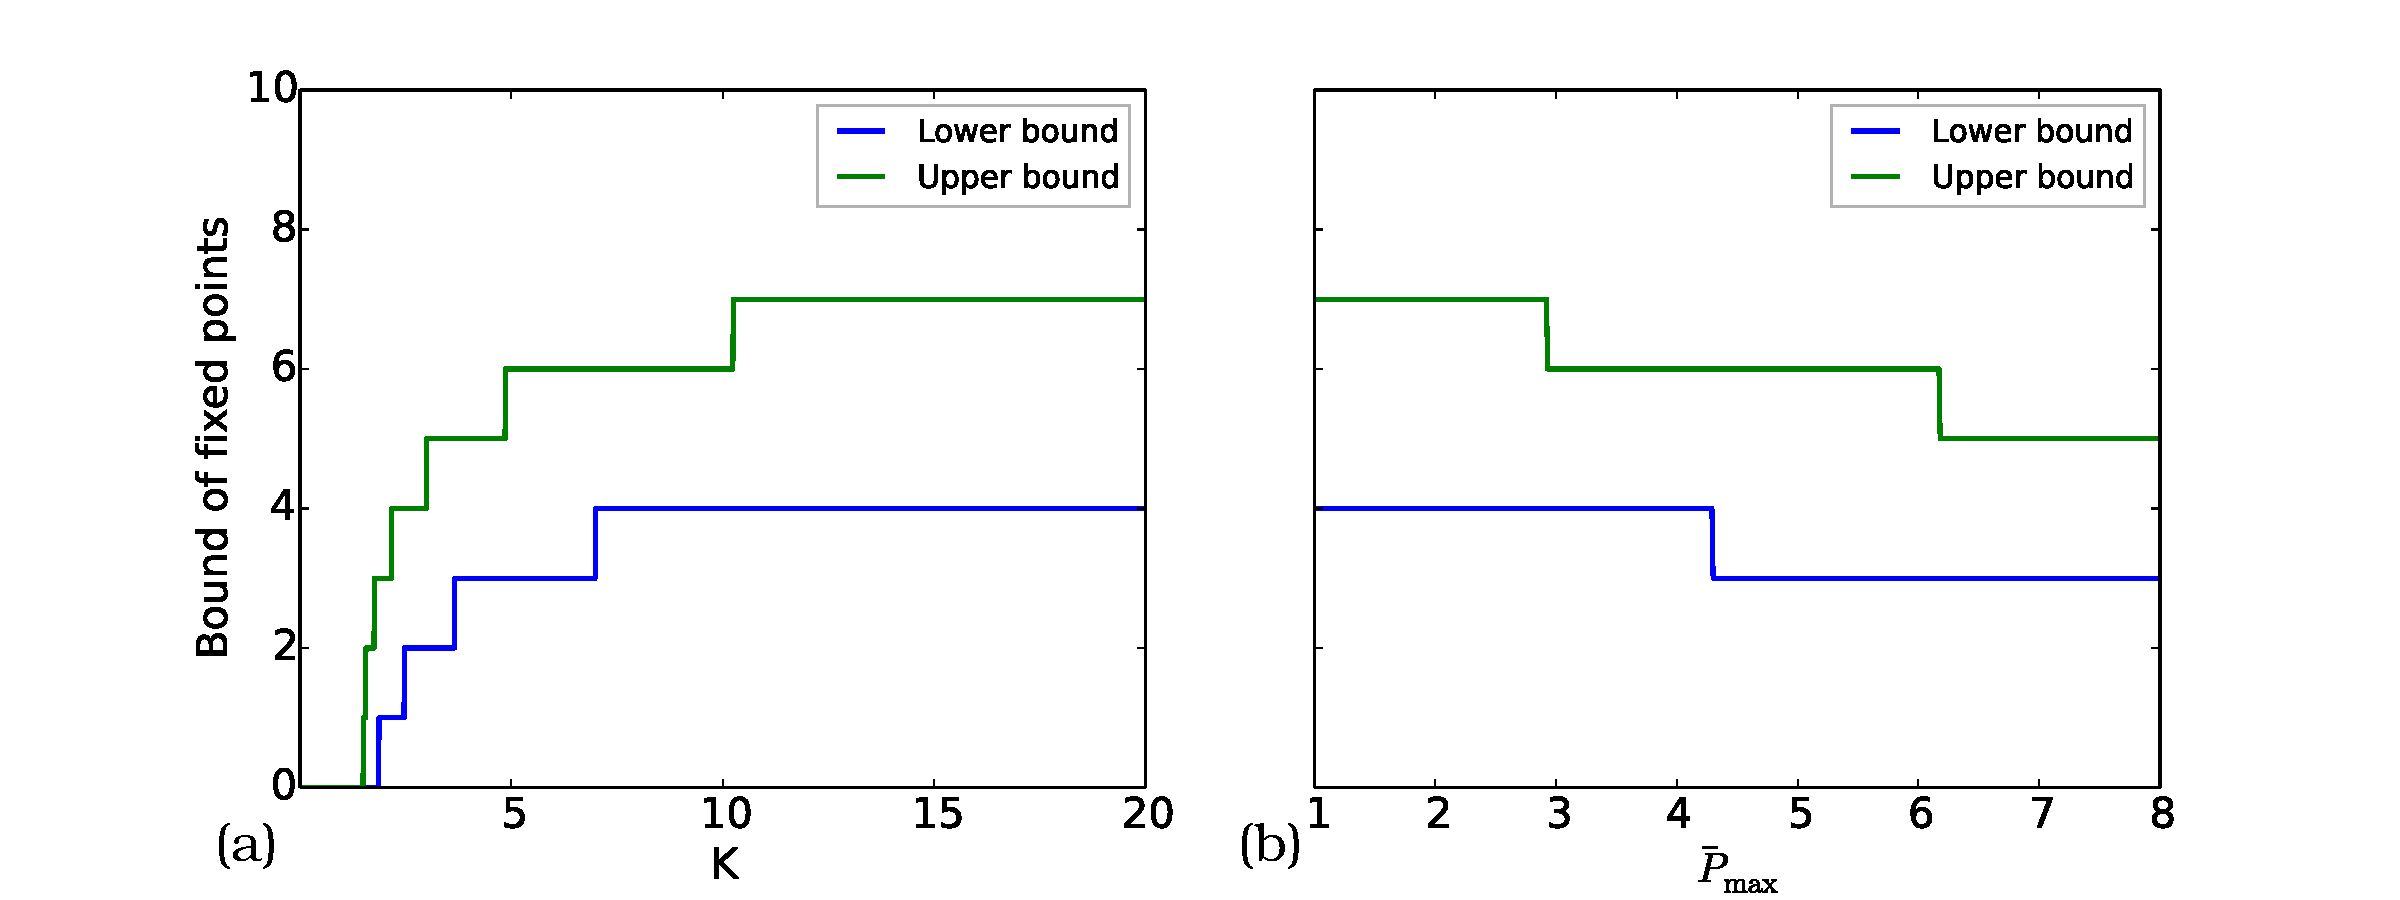
\includegraphics[width=\columnwidth]{pics/num_fps_k_p_ring}
\caption{
Upper and lower bounds for the number of steady states $N_f$ 
for a sample 16 element ring as a function of (a) $K$, which is same for all 
edges, while $\bar{P}_{\max}=3$, and (b) $\bar{P}_{\max}$ while $K=10$.  }
\end{center}
\end{figure}

We illustrate how the bounds scale with the connectivity $K$  and $\bar{P}_{\max}$ for a sample ring 
of size $16$ in  Fig \ref{fig:scaling-nf}. We see in Fig \ref{fig:scaling-nf} 
(a) that increasing $K$ results in more stable fixed points.  Whereas Fig 
\ref{fig:scaling-nf} (b)  demonstrates that if the power generators 
$(P_j\ge  0)$ are clustered together, then the system has less fixed points, 
as opposed to the case where they are more distributed.   


\subsection{Disproving established literature}
\debsankha{TODO}
Barahona et al claimed things that are not true.  

\subsection{More corrolaries}
\begin{lemma}
\label{}
Number of fixed points scales with the average length of cycles.  
\end{lemma}


\begin{corr}
\label{cor:high-k-nf}
A homogeneous ring network $R_{N}$ with $N$ nodes 
 will have multiple stable fixed 
points if 
\begin{align}
\label{crit:mult-fp}
K\geq \frac{\bar{P}_{\max}}{2\left(1-\frac{\pi}{N}\right)}
\end{align}
\end{corr}



\begin{corr}
\label{corr:nomult-3}
A homogeneous ring network of sixe $N$ doesn't have multiple fixed point for 
$N\leq 3$.  
\end{corr}

\begin{corr}
As $K$ is decreased, the fixed points with higher \emph{winding number} 
\eqref{eqn:gc2} will vanish. From another point of view, the fixed points with 
largest infinity norm
\[
\max_j\left|F_{j,j+1}\right|
\]
will be the first ones to vanish.  
\end{corr} 

\begin{lemma}
In a Kuramoto network, critical coupling scales as:
\[
K_c\propto \frac{\sum P_j}{N_E}
\]

Numerics approaches: \\
a. Devise an algorithm to calculate the RHS.   \\
b. Generate graphs suitably so that RHS is trivial to compute.  
\end{lemma}



\dirk{XXX Discussion: Similar results by [Ochab+Gora]. Compare!
}

\subsection{Complex networks}

\begin{defn}
For a connected  graph $G(V,E)$, we define a \emph{simple cycle set} $F$ as an 
ordered set containing the basis cycles of $G$
\[
F=\left[C_1, C_2,\cdots, C_{\gamma} \right],
\]
where 
\[
C_l=\left[v_{l1},v_{l2},\cdots, v_{ln}\right]
\]
%Without loss of generality, we order the nodes in a cycle $C_l$ in 
%counter-clockwise manner.   


It can be shown that 
$|F|=\gamma=|E|-|V|+1$ (cf. \debsankha{add ref}).  
\end{defn}


\begin{lemma}
\label{lem:cf-fp-corr-planar}
Let $\mathbf{S}_G$ be the set of all fixed points of a network $G$ 
satisfying the normal operation criteria \eqref{def:normalop}.
Then there exists a one-to-one function $\vec{f_c}:\mathbf{S}_R\mapsto \mathbf{R}^{\gamma}$ 
that maps each fixed point to a \emph{cycle flow vector}.  

\end{lemma}
\begin{proof}
Using the identical reasoning used in Lemma \ref{lem:cf-fp-corr} to arbitrary 
graphs instead of simple cycle, the proof follows.  
\end{proof}


\subsubsection{Planar graphs}
For planar graphs one can generalize the results of the section \ref{sec:cycles} in 
a straightforward way. To this end we define certain relevant quantities.  

\begin{defn}
\label{def:wvec}
For a connected planar graph $G$, and a certain distribution of generators $\vec{P}$, let $\vec{\phi^*}\in \mathbb{R}^{|V|}$ be a 
steady state.  Then the \emph{winding vector} $\vec{\omega}(\vec{\phi^*})$ is defined as:

\begin{align*}
\omega_l &= \frac{1}{2\pi} \sum_{e\in C_l} \arcsin{\frac{F_e}{K_e}}, \quad \forall 1 \leq l 
\leq \gamma\\
&=\frac{1}{2\pi} \sum_{e\in C_l} \arcsin{\frac{F_e^0+f^{cycle}_l-f^{cycle}_{n(e)}}{K_e}}
\end{align*}
\end{defn}

Here we have used the notation that for every edge $e\in C_l$, $n(e)$ is the 
index of the cycle adjacent to $C_l$ sharing edge $e$.  


\begin{lemma}
\label{lem:wind-fp-corr-planar}
For a planar network, if $\vec{\omega}(\vec{\phi_1})=\vec{\omega}(\vec{\phi_2})$ and both 
$\vec{\phi_1}$ and $\vec{\phi_2}$ satisfy \eqref{def:normalop} then 
\begin{align}
\label{}
\vec{\phi_1}&=\vec{\phi_2}. 
\end{align}
\end{lemma}

\begin{proof}
Suppose to the contrary.   

Let $\vec{f}$ and $\vec{f'}$ be the two cycleflow vectors as defined in 
\ref{lem:cf-fp-corr-planar} for $\vec{\phi_1}$ and $\vec{\phi_2}$ 
respectively.   

%Then, by virtue of our assumption 


Now consider the difference in cycleflows in each cycle between the two fixed points
\[
\{f'_l-f_l:1\leq l \leq \gamma\}
\]

Let $C_k$ be the cycle for which this quantity is largest

\begin{align}
\label{}
f'_k-f_k & \geq f'_l-f_l,\quad \forall l\neq k.  
\end{align}

Then we have

\begin{align}
\label{}
f'_k-f'_{n(e)} & \geq f_k-f_{n(e)} \quad\forall e\in C_k\\
\sum_{e\in C_k} \arcsin{\frac{F_e^0+f'_k-f'_{n(e)}}{K_e}} &\geq \sum_{e\in C_l} \arcsin{\frac{F_e^0+f_k-f_{n(e)}}{K_e}}\\
\Rightarrow \vec\omega_l(\vec{\phi_1})&\neq 
\vec\omega_l(\vec{\phi_2})\quad\text{ (using Definition \ref{def:wvec})}
\end{align}

This contradicts our contrary assumption.   
This concludes the proof.  
\end{proof}
 


\begin{lemma}
\label{}
Let $G$ be a planar network with simple cycle set $F=[C_1,C_2,\cdots,C_{\gamma}]$. Let $l_b$ be the length of the \emph{boundary} 
of $G$, i.e. the number of edges that are part of only one cycle.  Let 
$\omega^{\max}_l$ and $\omega^{\min}_l$ be the maximum and minimum winding 
number respectively for each cycle $C_l\in F$, as determined by \eqref{eq:lim-omega}.

Then the number of fixed points of a planar network is given by the total number of 
integer solutions to the linear inequality
\begin{align}
\label{}
-\frac{l_b}{4} \leq \sum_{l=1}^{\gamma} \omega_l \leq \frac{l_b}{4},
\end{align}
subject to the constraints
\begin{align}
\label{}
\omega^{\min}_l \leq \omega_l \leq \omega^{\max}_l.  
\end{align}
\end{lemma}



\subsubsection{Complete graph}
\begin{theorem}
\label{}
A completely connected network $G(n)$ has only one fixed point satisfying 
\eqref{def:normalop}. 
\end{theorem}

\begin{proof}
Since $G(n)$ is completely connected, we can choose simple cycle set $F$ of to 
consist of triangles, for example:
\[
F=[(n_1, n_2, n_3), (n_2,n_3,n_4),\cdots, ].
\]

Suppose $\vec{\phi^*}$ is a fixed point of a completely connected network.   
From Lemma \ref{lem:cf-fp-corr-planar}, we see that any other fixed point, if 
it exists, must consist of cycleflows in the triangles that make up $F$.   
Now, in order to satisfy \eqref{def:normalop}, the new cycleflows must cause the 
phase difference along the cycle to change by a multiple of $2\pi$.  

However, since phase difference along an edge can be maximally $\frac{\pi}{2}$ 
as per our constraint \eqref{def:normalop}, the phase difference in the whole 
cycle can change by at most $\frac{3\pi}{2}$.   

Therefore another fixed point cannot exist in a completely connected network.  
\end{proof}



\section{Conclusion}



\textbf{XXX Marc XXX}




% --- Literatur -------------------------------------------------------------------

\bibliography{networks,power,publwi,kuramoto}
\bibliographystyle{apsrev}


\end{document}
